\chapter{Stilvorgaben}
\section{Allgemeine Stilvorgaben}


% Ok
Unter dem Satzspiegel wird die vom gew�hnlichen Text inklusive Fu�noten und von den Abbildungen bzw. Tabellen eingenommene Fl�che einer bedruckten Seite verstanden. Sonstige Angaben und Textzus�tze wie etwa eine Kopf- oder Fu�zeile und die Seitenzahlen (Pagina) geh�ren nicht zum Satzspiegel und laufen au�erhalb dieses Raumes.

% Ok
F�r Arbeiten an der EUFH sind f�r den Satzspiegel folgende Ma�e verbindlich: Der linke Rand muss 2,5 cm, der rechte Seitenrand 3,5 cm, der obere Rand 2,5 cm und der untere Rand 2 cm breit gew�hlt werden.



[\ldots] 

% Ok
Die Nummerierung wird �blicherweise in einer einzeiligen Kopfzeile - mittig oder rechts - vorgenommen. 
% Nicht ok
Titel- bzw. Deckblatt werden bei der Seitennummerierung mitgez�hlt, aber nicht paginiert. Der Text beginnt mit der Einleitung (Seite 1) und wird mit arabischen Ziffern nummeriert; f�r die zuvor vorhandenen Verzeichnisse wird eine r�mische Seitennummerierung verwendet, f�r die Verzeichnisse danach wird die Nummerierung mit arabischen Ziffern fortgef�hrt.
 
% Ok
[\ldots] Als Grundschriftart wird Times New Roman eingesetzt. Arial ist gut geeignet f�r �berschriften. Als Schriftgr��e ist 12 Punkt zu w�hlen. F�r die Titelseite werden auch andere Schriftgrade eingesetzt. In Arbeiten wird standardm��ig ein Zeilenabstand von 1,5 Zeilen verwendet. Der Standardtext wird im Blocksatz ausgerichtet.

% Nicht ok
Vor �berschriften empfiehlt sich ein Abstand, der eineinhalb bis zweimal so gro� ist wie der Abstand von der �berschrift zum darauf folgenden Text. Mathematische Formeln werden �blicherweise linksb�ndig einger�ckt und rechtsb�ndig nummeriert.

[\ldots]

% Nicht ok
Jedes Kapitel der ersten Gliederungsebene sollte nach M�glichkeit auf einer neuen Seite beginnen. Bei Seitenumbr�chen ist des Weiteren zu beachten, dass keine einzelnen Zeilen eines Absatzes auf der folgenden oder der vorangehenden Seite entstehen. Die vereinsamte erste Zeile eines Absatzes auf dem unteren Ende der Seite wird im Fachjargon Schusterjunge genannt; Hurenkind wird die letzte Zeile eines Absatzes auf der folgenden Seite genannt.


\chapter{Beispiele}

\section{Literaturquellen}


Wir zeigen Beispiele von Quellverweise auf ein Buch (\cite{heinrich2011wirtschaftsinformatik}),
einen Zeitschriftenbeitrag (\cite{wilde2007forschungsmethoden}),
einen Konferenzbeitrag (\cite{schauer2008wirtschaftsinformatik}),
einen Buchbeitrag (\cite{chamoni2019wirtschaftsinformatik}, Sonderfall, weil online ver�ffentlicht)),
eine Doktorarbeit (\cite{gabriel1979programmierungsprobleme})
und einen Forschungsreport (\cite{scheer2003geschaftsmodelle}). Das gleiche geht auch alles mit technischen Reports und Fu�noten\footnote{Vgl. \cite{lehman2022biblatex}.}. 

Ein (nicht empfohlenes, aber formal korrektes) indirektes Zitat zeigen wir in der Fu�note auf Seite \pageref{text:indirektesZitat}.









\newpage
\section{Abbildungen, Tabellen, Formeln}

\subsection{Abbildungen}
Wir sehen ein Beispiel einer Abbildungen (\ref{fig:umwegmodell} auf Seite \pageref{fig:umwegmodell}). 


\begin{figure}
  \centering
  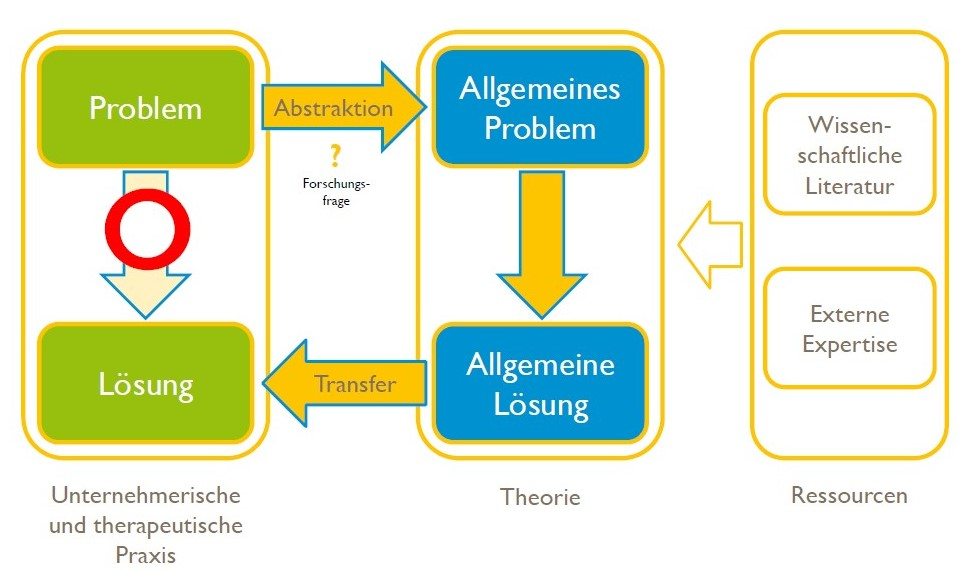
\includegraphics[width=.8\textwidth]{abbildungen/umwegmodell}
  \caption{Umwegmodell}
  \label{fig:umwegmodell}
\end{figure}

\newpage
\subsection{Tabellen}
Wir sehen ein Beispiel einer Tabelle (\ref{tab:beispielstabelle} auf Seite \pageref{tab:beispielstabelle}).

\begin{table}
\centering
\begin{tabular}{lll}
\toprule

�berschrift 1 & �berschrift 2	& �berschrift 3	\\

\midrule

Lorem ipsum & dolor sit amet & consetetur sadipscing \\
elitr, sed diam  & nonumy eirmod tempor & invidunt ut labore et \\
dolore magna aliquyam &  erat, sed diam  & voluptua.  \\

\bottomrule
\end{tabular}
\caption{Beispielstabelle}
\label{tab:beispielstabelle}
\end{table}

\newpage
\subsection{Formeln}

Wir sehen als Beispiel einer Formel die Berechnung einer Stichprobe f�r eine Grundgesamtheit unter 100.000 (\ref{formula:stichprobenumfang} auf Seite \pageref{formula:stichprobenumfang}\footnote{\label{text:indirektesZitat}Vgl. \cite{hinterhuber1997kundenzufriedenheit}, S. 75f. zitiert nach \cite{kornmeier2007wissenschaftstheorie}, S. 163.}). Formeln k�nnen ebenfalls in den Flie�text integriert werden: $n = \frac{t^2 * p * q * N}{t^2 * p * q + e^2 * (N-1)}$.

\begin{equation}
n = \frac{t^2 * p * q * N}{t^2 * p * q + e^2 * (N-1)}
\label{formula:stichprobenumfang}
\end{equation}

\newpage
\section{Blindtexte}

%%%%%%%%%%%%%%%%%%%%%%%%%%%%%%%%%%%%%%%%%%
Lorem ipsum dolor sit amet, consetetur sadipscing elitr, sed diam nonumy eirmod tempor invidunt ut labore et dolore magna aliquyam erat, sed diam voluptua. At vero eos et accusam et justo duo dolores et ea rebum. Stet clita kasd gubergren, no sea takimata sanctus est Lorem ipsum dolor sit amet. Lorem ipsum dolor sit amet, consetetur sadipscing elitr, sed diam nonumy eirmod tempor invidunt ut labore et dolore magna aliquyam erat, sed diam voluptua. At vero eos et accusam et justo duo dolores et ea rebum. Stet clita kasd gubergren, no sea takimata sanctus est Lorem ipsum dolor sit amet. Lorem ipsum dolor sit amet, consetetur sadipscing elitr, sed diam nonumy eirmod tempor invidunt ut labore et dolore magna aliquyam erat, sed diam voluptua. At vero eos et accusam et justo duo dolores et ea rebum. Stet clita kasd gubergren, no sea takimata sanctus est Lorem ipsum dolor sit amet. 

Duis autem vel eum iriure dolor in hendrerit in vulputate velit esse molestie consequat, vel illum dolore eu feugiat nulla facilisis at vero eros et accumsan et iusto odio dignissim qui blandit praesent luptatum zzril delenit augue duis dolore te feugait nulla facilisi. Lorem ipsum dolor sit amet, consectetuer adipiscing elit, sed diam nonummy nibh euismod tincidunt ut laoreet dolore magna aliquam erat volutpat. 

Ut wisi enim ad minim veniam, quis nostrud exerci tation ullamcorper suscipit lobortis nisl ut aliquip ex ea commodo consequat. Duis autem vel eum iriure dolor in hendrerit in vulputate velit esse molestie consequat, vel illum dolore eu feugiat nulla facilisis at vero eros et accumsan et iusto odio dignissim qui blandit praesent luptatum zzril delenit augue duis dolore te feugait nulla facilisi.